\documentclass[./skripsi.tex]{subfiles}
\begin{document}
\chapter{Metode Penelitian}
\section{Metode Penelitian}
Metode penelitian yang digunakan pada penelitian ini adalah metode penelitian kuantitatif deskriptif. Berikut adalah gambaran penelitian yang diusulkan.
\begin{center}
\makebox {
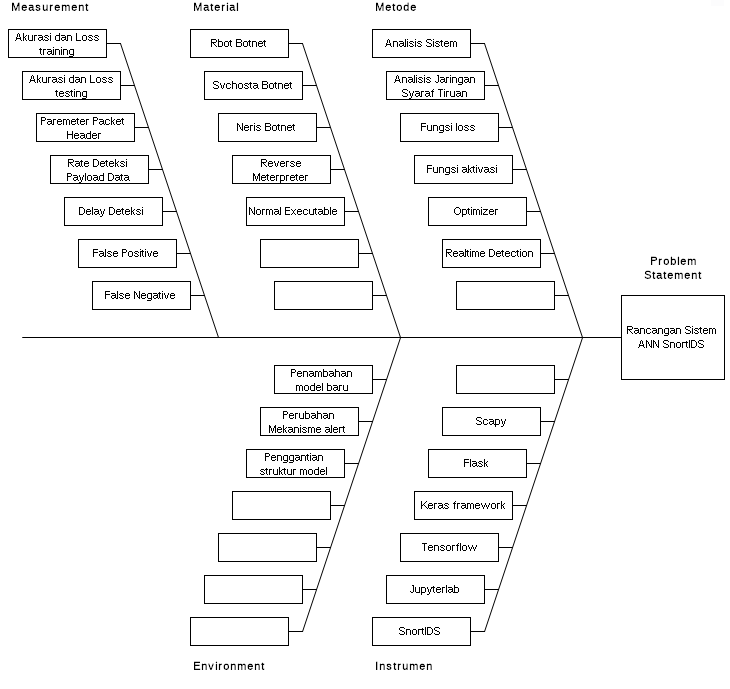
\includegraphics[width=0.8\textwidth]{skripsi/public/assets/img/fishbonepenelitian.png}
}
\captionof{figure}{Metode Penelitian}\label{svc_loss}
\end{center}
\section{Waktu dan Tempat Pelaksanaan}
\par Waktu dan tempat pelaksanaan penelitian ini adalah sebagai berikut :
\subsection{Waktu Pelaksanaan}
%Disini mulai%

%Disini selesai%
\par Waktu pelaksanaan penelitian dilakukan dari tanggal 1 Maret 2019 sampai dengan 31 Juli 2019.
\subsection{Tempat Pelaksanaan}
\par Pelaksanaan penelitian dilakukan di Laboratorium 3 UPT Pusat Teknologi Informasi dan Komunikasi Universitas Mataram
\section{Populasi dan Sampel}
\par Populasi dan sampel penelitian ini adalah sebagai berikut :
\subsection{Populasi Penelitian}
\par Populasi pada penelitian ini mencakup intrusi dalam bentuk Executable-based Virus dan Payload-based Virus
\subsection{Sampel Penelitian}
\par Sampel pada penelitian ini antara lain :
\begin{enumerate}
    \item Neris Botnet executable
    \item Neris Botnet Traffic Data pcap
    \item RBot Botnet executable
    \item RBot Botnet Traffic Data pcap
    \item Svchosta Botnet executable
    \item Svchosta Botnet Traffic Data pcap
    \item Payload Reverse Meterpreter dalam file PE32
    \item File executable normal
\end{enumerate}
\section{Instrumen Penelitian}
Instrumen penelitian yang digunakan antara lain :
\begin{enumerate}
    \item SnortIDS sebagai Intrusion Detection System
    \item Python sebagai bahasa pemrograman yang digunakan untuk deteksi intrusi
    \item Library python seperti : tensorflow, keras, numpy, matplotlib untuk perlengkapan pada saat training data dan testing data dengan Convolutional Neural Network dan Long Short Term Memory.
    \item Python flask sebagai library untuk webservice filter
    \item PC Server Linux sebagai host yang menjalankan SnortIDS, dan Python
\end{enumerate}
\subsection{Proses Pengembangan Instrumen}
\par Proses pengembangan instrumen berawal dari perancangan instrumen, uji validitas instrumen, Uji reliabilitas instrumen.
\subsection{Uji Validitas Instrumen}
\par Proses pengujian validitas instrumen dilakukan dengan menguji IDS dengan data input yang sama, lalu mengamati hasilnya yang kemudian akan disesuaikan.
\subsubsection{Hasil Uji Validitas Instrumen}
\par Isinya tabel training data di Jupyterlab
\subsection{Uji Reliabilitas Instrumen}
\par Proses pengujian reliabilitas instrumen dilakukan dengan menguji IDS dengan data input yang bervariasi
\subsubsection{Hasil Uji Reliabilitas Instrumen}
\par Isinya proses testing pada snortIDS
\section{Prosedur Penelitian}
\par Prosedur penelitian terdiri dari Perancangan sistem training dan perancangan sistem filter untuk testing. Rancangan sistem training dibuat dengan menggunakan jupyter notebook. Sedangkan Rancangan sistem filter menggunakan snortIDS dan flask framework untuk menghubungkan keluaran data dari snortIDS ke dalam model CNN dan LSTM.
\subsection{Perancangan Sistem}
\par Rancangan sistem filter terdiri dari Dataset yang dijadikan data untuk proses testing. Pada sisi filter juga terdapat IP\_buffer yang digunakan sebagai input yang akan mengumpulkan packet yang bersumber dari alamat IP yang sama.
\par Alamat IP yang berbeda-beda atau berubah-ubah dapat diketahui dari kemiripan transmisi header antara satu packet dengan packet lain. Jika kemiripan nya tinggi maka akan dianggap alamat IP diubah-ubah atau terindikasi Denial of Service.
\begin{center}
\makebox {
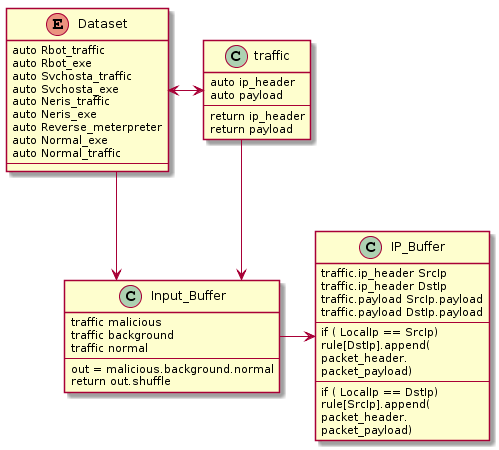
\includegraphics[width=0.5\textwidth]{skripsi/public/assets/img/RancanganSistemPenelitian.png}
}
\captionof{figure}{Model Rancangan Sistem}\label{svc_loss}
\end{center}
\section{Analisis Data}
\par Proses analisis data meliputi analisis tabel dan analisis grafis dari seluruh hasil pengujian validitas dan reliabilitas instrumen
\subsection{Prosedur Pengolahan Data}
\par Pengolahan data dilakukan dengan menyesuaikan bentuk input data dengan bentuk input yang diharapkan neuron sebelum dilakukan training.

\begin{table}[!htbp]
\centering
\caption{Data hasil pengukuran CNN}
\begin{tabular}{|l|l|l|l|l|l|l|}
\hline
\textbf{No} & \textbf{Input} & \multicolumn{1}{c|}{\textbf{\begin{tabular}[c]{@{}c@{}}Akurasi \\ Training\end{tabular}}} & \multicolumn{1}{c|}{\textbf{\begin{tabular}[c]{@{}c@{}}Loss\\ Training\end{tabular}}} & \multicolumn{1}{c|}{\textbf{\begin{tabular}[c]{@{}c@{}}Akurasi \\ Testing\end{tabular}}} & \multicolumn{1}{c|}{\textbf{\begin{tabular}[c]{@{}c@{}}Loss \\ Testing\end{tabular}}} & \multicolumn{1}{c|}{\textbf{\begin{tabular}[c]{@{}c@{}}Rate \\ deteksi\end{tabular}}} \\ \hline
1 & Neris Botnet &  &  &  &  &  \\ \hline
2 & RBot Botnet &  &  &  &  &  \\ \hline
3 & Svchosta Botnet &  &  &  &  &  \\ \hline
4 & Single Payload &  &  &  &  &  \\ \hline
5 & Multi Payload &  &  &  &  &  \\ \hline
\end{tabular}
\end{table}

\begin{table}[h]
\centering
\caption{Data Hasil untuk SnortIDS}
\begin{tabular}{|l|l|l|l|l|l|l|}
\hline
\textbf{No} & \textbf{Input} & \multicolumn{1}{c|}{\textbf{\begin{tabular}[c]{@{}c@{}}n Packet\\ Terdeteksi\end{tabular}}} & \multicolumn{1}{c|}{\textbf{\begin{tabular}[c]{@{}c@{}}n Packet\\ Lolos\end{tabular}}} & \multicolumn{1}{c|}{\textbf{\begin{tabular}[c]{@{}c@{}}False\\ Positive\end{tabular}}} & \multicolumn{1}{c|}{\textbf{\begin{tabular}[c]{@{}c@{}}False\\ Negative\end{tabular}}} & \multicolumn{1}{c|}{\textbf{\begin{tabular}[c]{@{}c@{}}Rate \\ Deteksi\end{tabular}}} \\ \hline
1 & Neris Botnet &  &  &  &  &  \\ \hline
2 & RBot Botnet &  &  &  &  &  \\ \hline
3 & Svchosta Botnet &  &  &  &  &  \\ \hline
4 & Firefox PE32 &  &  &  &  &  \\ \hline
5 & Single PE32 &  &  &  &  &  \\ \hline
6 & Multi PE32 &  &  &  &  &  \\ \hline
\end{tabular}
\end{table}
\subsection{Teknik Analisis Data}
\par Data dianalisis pada sisi akurasi, loss, dan rate pendeteksian pada SnortIDS. Dicari tingkat konvergensi dan bentuk model yang dipakai untuk tiap-tiap kelas BotNet.
\subsection{Membuat klastering data}
\par Data kelas terbagi menjadi 2 yakni \texit{Malicious} dan \textit{Benign}. Untuk membedakan kedua kelas ini dilakukan training pada data \textit{malicious} dengan dua kelas.
\end{document}